\documentclass{beamer}
\usepackage{ngerman}
\usepackage{beamerthemesplit}
\usepackage[ansinew]{inputenc}
\usepackage{ngerman}
\usepackage[T1]{fontenc}
%\usepackage{colortbl}
\usepackage{pgf,pgfnodes,pgfautomata,pgfheaps,pgfshade}

\usepackage{hyperref}
\usepackage{natbib}
\def\newblock{\hskip .11em plus.33em minus.07em}


\logo{\pgfimage[width=0.8cm,hight=0.8cm]{EURACE_Flag}}

\title{The Production Sector in EURACE}
\subtitle{EURACE Winter School 2009}
\author{H. Dawid, S. Gemkow, P.
Harting, and M. Neugart}

\begin{document}
\begin{frame}{}
\centering
\includegraphics[scale=0.1]{EURACE_Flag.png}
\titlepage
\end{frame}

\section[Overview]{}
\frame{\tableofcontents}

\section{Introduction}





\frame
{
  \frametitle{The real side of EURACE} 

%\begin{itemize}

%\item 3 real markets in EURACE:
		
%		\begin{itemize}
%				\item Consumption Goods Market.
%				\begin{itemize}
%					\item Production and selling of a homogeneous consumption good.
		
%		\end{itemize}
		
%		\item Capital Goods Market.
		
%	\begin{itemize}
%		\item Capital goods are vertically differentiated among their productivity. 
	
	 

%	\end{itemize}
%		\item Labor Market.
%		\begin{itemize}
%	\item  Labor differentiated among general and specific skills.

%\end{itemize}

%	\item Labor and capital goods are input factors for the production of the consumption good.

%		\end{itemize}
%\end{itemize}	



\begin{itemize}
	\item The core of the Production Sector: Consumption Goods Market
	
\begin{itemize}
	\item Production and selling of a homogeneous consumption good.

\end{itemize}

	\item 2 Factor Markets:
	
\begin{itemize}
	\item Capital Goods Market: 
	
\begin{itemize}
	\item Capital goods are vertically differentiated among their productivity.
\end{itemize}

\item Labor Market:
\begin{itemize}
	\item Labor differentiated among general and specific skills.
\end{itemize}
\end{itemize}


\end{itemize}
}
%%%%%%%%%%%%%%%%%%%%%%%%%%%%%%%%%%%%%%%%%%%%%%%%%%%%%%%%%%%%%%%%%%%%%%%%%%%%%%%%%%%%%%%%%%%%%%%%%%%%%%%%%%%%%

\frame
{
  \frametitle{Agents and their roles} 
\begin{itemize}
	\item Consumption goods producer:
	
\begin{itemize}
	\item Producer and seller of consumption goods.
	\item Buyer of labor and capital goods. 
\end{itemize}

	\item Households:
	
\begin{itemize}
	\item Consumer on the Consumption Goods Market.
	\item Supplier on the Labor Market.
\end{itemize}

\item Investment Goods Producer:

\begin{itemize}
	\item Supplier on the Investment Goods Market.
\end{itemize}

\item Malls (passive agent type):

\begin{itemize}
	\item Market platforms where consumption goods producers store and offer their commodities.
	\item Transfer of information and goods between producers and consumers.
\end{itemize}
	
\end{itemize}
	

}

\frame
{
  \frametitle{Regional structure} 
\begin{itemize}
	\item Consumption Goods Market: Semi local market
	
\begin{itemize}
	\item On the supply side the market is global: producers can deliver goods
to all malls.
	\item On the demand side the CGM is a local market: consumers shop in their region
\end{itemize}

\item Investment Goods Market: Global market
\begin{itemize}
	\item  All firms have frictionless access to the IG market.
\end{itemize}
\item Labor Market: Semi local market
\begin{itemize}
	\item Firms can hire workers from their home region and neighboring regions.
	\item Workers have to bear commuting costs if they work for firms in outside regions. 
\end{itemize}


	
\end{itemize}
	

}



%%%%%%%%%%%%%%%%%%%%%%%%%%%%%%%%%%%%%%%%%%%%%%%%%%%%%%%%%%%%%%%%%%%%%%%%%%%%%%%%%%%%%%%%%%%%%%%%%%%%%%%%%%%%%



\frame
{
  \frametitle{General modeling philosophy} 
\begin{itemize}
\item Strong micro-foundation of decision rules:
 firms and households act rule-based using backward looking expectations. 

\item Operational decisions of firms are modeled using standard decision rules from the Operations Management literature: 
\begin{itemize}
	\item Pricing (markup)
\item Inventory and production planing (newsboy problem)
\end{itemize}

\item Savings/consumption decisions of HHs are simplified versions of empirically confirmed rules.

	
\end{itemize}


}


%%%%%%%%%%%%%%%%%%%%%%%%%%%%%%%%%%%%%%%%%%%%%%%%%%%%%%%%%%%%%%%%%%%%%%%%%%%%%%%%%%%%%%%%%%%%%%%%%%%%%%%%%%%%%%%%%%

\section{The Consumption Goods Producer}


%%%%%%%%%%%%%%%%%%%%%%%%%%%%%%%%%%%%%%%%%%%%%%%%%%%%%%%%%%%%%%%%%%%%%%%%%%%%%%%%%%%%%%%%%%%%%%%%%%%%%%%%%%%%%%%%%%

\frame
{
  \frametitle{General features} 
\begin{itemize}
	\item The firm uses capital and labor to produce consumption goods.
	\item Firms are located in regions.
		
\begin{itemize}
	\item The commodities are sold at geographically distributed outlet malls.
	\item Goods can be frictionless transfered to all regions/malls.
	\item Firms have access to the (global) Investment Goods Market.
	\item There are barriers to hire workers from outside regions (commuting costs).
\end{itemize}

	\item The firm can finance the production and investments internally and externally.
	\end{itemize}


}


\frame
{
 \frametitle{} 
\begin{figure}
\centering
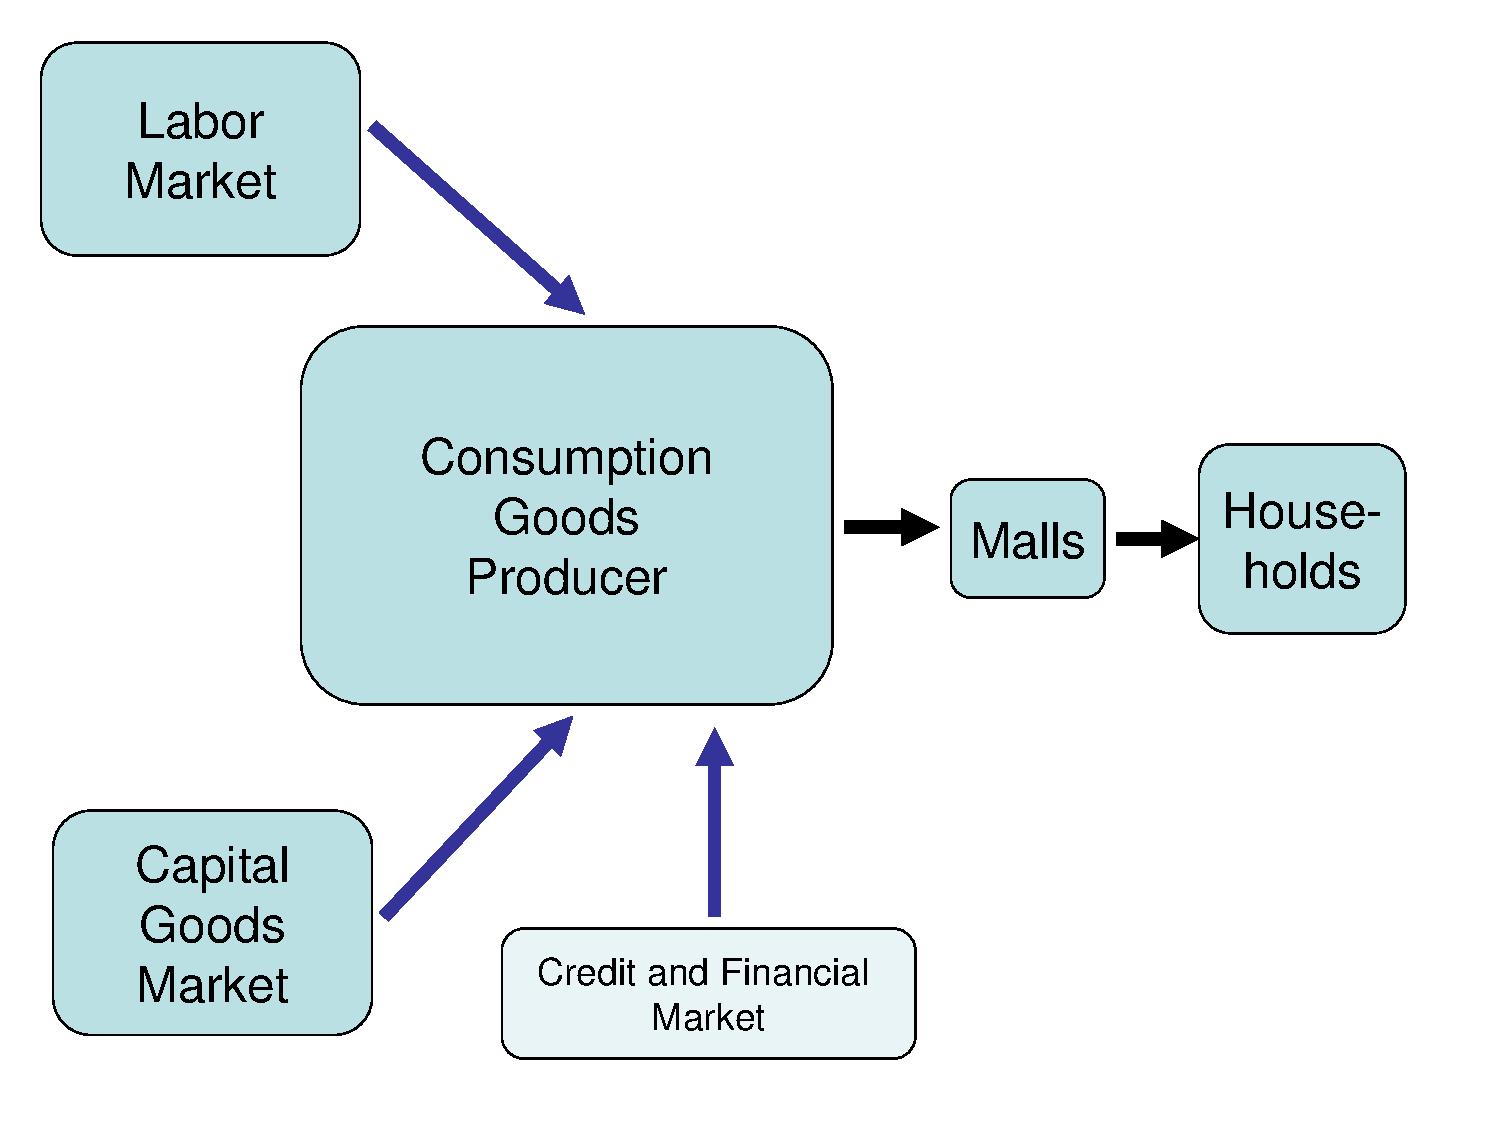
\includegraphics[scale=0.35]{CGP_Overview.pdf}
\label{fig:CGP_Overview}
\end{figure}


}

\frame
{
  \frametitle{Technology} 
\begin{itemize}
	\item The production technology of firm $i$ is embedded in firm's capital stock $K_{i,t}$ and is characterized by its 		technical productivity $A_{i,t}$.
\begin{itemize}
 	\item Provided by capital goods producers with a quality that increases over time.
\end{itemize}
		\item Average productivity $A_{i,t}$ of the capital stock depends on past investments.
		\item $A_{i,t}$ is updated by depreciation and new physical investments.
		\item The firm depreciates its capital stock $K_{i,t}$ at a rate $\delta$, it follows $K_{i,t}=(1-\delta)K_{i,t-1}+I_{i,t}$.
	\end{itemize}
}


%%%%%%%%%%%%%%%%%%%%%%%%%%%%%%%%%%%%%%%%%%%%%%%%%%%%%%%%%%%%%%%%%%%%%%%%%%%%%%%%%%%%%%%%%%%%%%%%%%%%%%%%%%%%%%%%
\frame{

\frametitle{The impact of Skills} 
\begin{itemize}
	\item A worker $w$ has two skill dimensions:
	\begin{itemize}
	\item General skills: Education and general abilities measured in 5 discrete skill groups $b_w^{gen}=\left\{1,...5\right\}.$
	\item Specific skills: $b_{w,t}$ are experiences and know how obtained on the job. 
	\item Specific skills of a worker $w$ employed in firm $i$ evolve through learning by doing etc. according to \[ b_{w,t}=b_{w,t-1}+ \chi (b_w^{gen})\cdot \max\left[0,(A_{i,t}-b_{w,t-1})\right]. \]
		
\begin{itemize}
	\item Building up specific skills depends on educational level. 
	\item Function $\chi$ increasing in the general skill level of worker $w$, $f'(b_w^{gen})>0$.
	 
\end{itemize}
\end{itemize}
\end{itemize}
}


%%%%%%%%%%%%%%%%%%%%%%%%%%%%%%%%%%%%%%%%%%%%%%%%%%%%%%%%%%%%%%%%%%%%%%%%%%%%%%%%%%%%%%%%%%%%%%%%%%%%%%%%%%%%%%%
\frame{

\frametitle{Interaction of Technology and Skills} 

\begin{itemize}
\item Complementarity between mean specific skills $B_{i,t}$ and technical productivity $A_{i,t}.$
\item Effective productivity $A^{eff}_{i,t}=\min \left[A_{i,t},B_{i,t}\right].$
\item Productivity of a given technology level is only fully exploited if workers in the firm have sufficiently high specific skills. 

	
\end{itemize}
 
}




\frame
{
  \frametitle{Production Function} 
\begin{itemize}
	\item Production Function of a Consumption Goods Producer:
	
	
\begin{itemize}
	
	\item Cobb-Douglas production function
	
	\[ Q_{i,t}=  \min \left[A_{i,t},B_{i,t}\right] L_{i,t}^{\alpha}K_{i,t}^{\beta}.\]
	
	\item $ L_{i,t}$ current labor stock, $ K_{i,t}$ capital stock, $\alpha, \beta$ input factor intensity with constant returns to scale, $\alpha + \beta =1$.

\end{itemize}

	\end{itemize}


}


\frame
{
  \frametitle{Sequence of activities} 


\begin{itemize}
	\item The sequence of decisions and actions
	\begin{itemize}
	\item Production planning.
	\item Tentative input factor planning.
	\item Financial planning.
	\item Final production planning and input factor determination.
	\item Labor and Capital Market transactions.
	\item Production and delivery.
	\item Periodic earnings statement.
	 
	\end{itemize}
	
	\end{itemize}


}

\frame
{
  \frametitle{Timing} 
  
  \begin{itemize}	
	\item Timing of production
	
\begin{itemize}
	\item Length of the production and selling cycle: 1 month. 
	\item At the monthly activation day (first day of the cycle): Production planing, financing, production, and delivery to the malls.
	\item Selling during the whole of the month.
	\item Earnings statement at the last day of the production cycle.
\end{itemize}
\end{itemize}


}


\frame
{
  \frametitle{Production planning} 
\begin{itemize}
	\item Standard inventory rule with stochastic demand: The firms compute different delivery volumes for all served malls (newsboy problem).
	
	\item $Y_{i,r,t}$ is the critical stock of firm $i$ in mall $r$, $SL_{i,r,t}$ is the current mall stock at the activation day.
		
	\item Desired replenishment quantity:
	\[
			\tilde{D}_{i,r,t}= \begin{cases} 0 & SL_{i,r,t}\geq Y_{i,r,t},\\
																			Y_{i,r,t} -  SL_{i,r,t} &else. 
			
			 \end{cases}
	\]
	
	
	\end{itemize}


}

\frame
{

  \frametitle{Production planning} 
\begin{itemize}

\item Demand is estimated by computing a linear trend from the previous demands.

\item Demand of the last $\tau$ periods for mall $r$: $\left\{ \hat{D}_{i,r,t-\tau},...,\hat{D}_{i,r,t-1} \right\}$.

\item Determination of the demand (Estimation with a simple adaption rule):  
		\[
				\hat{D}_{i,r,t}=\begin{cases}  S_{i,r,t} & if SL_{i,r,t}>0 \\ S_{i,r,t}\cdot (1+ \nu) & if SL_{i,r,t}=0, \end{cases}
		\]
		where $0 < \nu < 1$ and $S_{i,r,t}$ is the sold quantity in mall $r$.
\end{itemize}
  
}


\frame
{
  \frametitle{Production planning} 
\begin{itemize}
	
	
	\item $Y_{i,r,t}$ is chosen such that the firm expects to be able to satisfy the market demand with probability $1-\chi$ ($\chi$ stock-out probability).
	
	\item Linear regression model based on previous demands:
	\[
			Y_{i,r,t}= \hat{a}_{i,r,t}+\tau \cdot \hat{b}_{i,r,t}+\bar{q}_{1-\chi}\cdot \sqrt{\hat{\delta}_{i,r,t}}.
	\]
	
	\item $\hat{a}, \hat{b}$ linear regression coefficients, $\hat{\delta}$ estimated variance, and $\bar{q}_{1-\chi}$ the $1-\chi$-quantile of the standard normal distribution. 
	\end{itemize}


}

\frame
{
 \frametitle{Production planning}
 
\begin{itemize}
	\item  Illustration: Linear regression of  $\hat{D}_{i,r,t-\tau+ s}$ with regressor $s$, and $\tau=10$ past observations. 
	\item Estimation of demand for $s=10:  \hat{D}_{i,r,t}=Y_{i,r,t}$ 
\end{itemize}
   
\begin{figure}
\centering
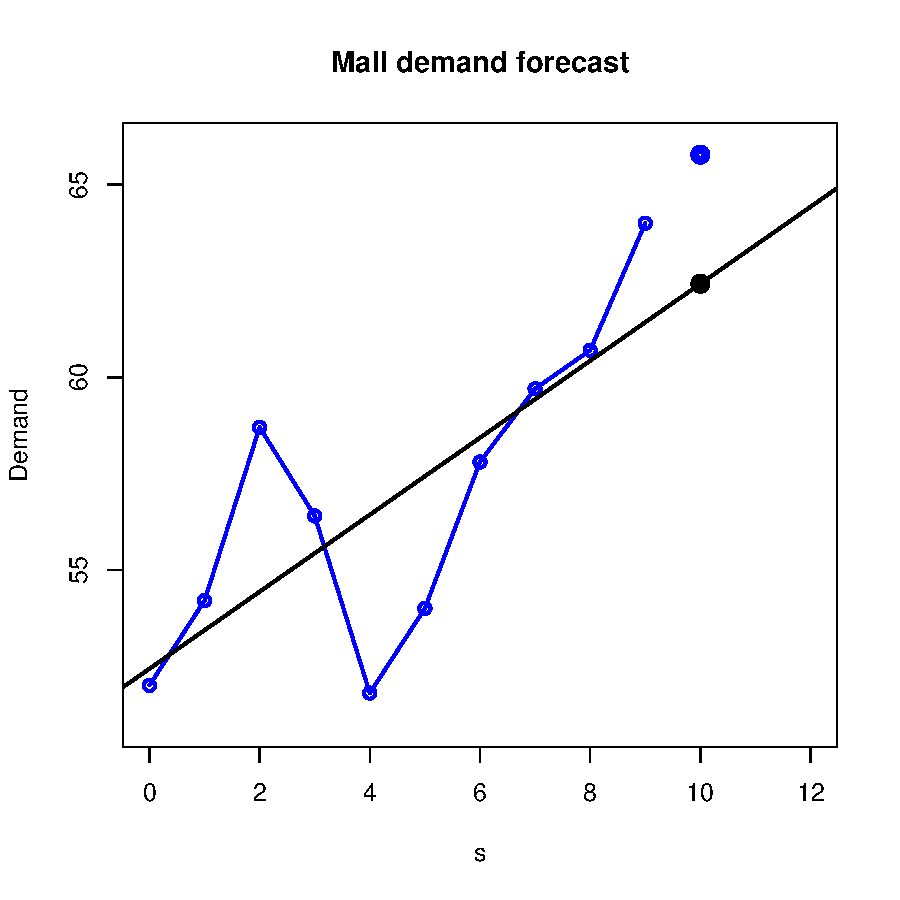
\includegraphics[scale=0.3]{regression.pdf}
\label{fig:regression}
\end{figure}



}


\frame
{
  \frametitle{Production planning} 
\begin{itemize}

\item Desired replenishment quantity:
	\[
			\tilde{D}_{i,r,t}= \begin{cases} 0 & SL_{i,r,t}\geq Y_{i,r,t},\\
																			Y_{i,r,t} -  SL_{i,r,t} &else. 
			
			 \end{cases}
	\]

	\item Sum of all replenishment quantities is $\tilde{D}_{i,t}=\sum{}_{r=1}^R \tilde{D}_{i,r,t}.$
	
	\item Smoothing of (planned) production quantity: 
	 \[
	 \tilde{Q}_{i,t}=\xi \tilde{D}_{i,t} + (1-\xi)\frac{1}{T}\sum_{k=t-T}^{t-1}\tilde{Q}_{i,k}.
	 \]
	
	\item Proportional adjustment of delivery volumes: $D_{i,r,t}=\frac{ \tilde{D}_{i,r,t}}{\tilde{D}_{i,t}}\tilde{Q}_{i,t}.$
	\end{itemize}


}



\frame
{

  \frametitle{Input factor planning} 
\begin{itemize}
	\item The firm aims to realize a capital to labor ratio according to the standard rule for CES production functions: 
		\[
	\frac{\tilde K_{i,t}}{p^{inv}} / \frac{\tilde L_{i,t}}{w_t^e} =\frac{\beta}{\alpha}.
	\]
	\item $w_t^e$ expected mean wage, and $p^{inv}$ a calculatory capital goods price.

	
	
	
\end{itemize}

}


\frame
{

  \frametitle{Input factor planning: Capital} 
\begin{itemize}

\item Optimal capital stock 
\[
\tilde {\tilde K}_{i,t}= \frac{(\beta w_t^e)^{\alpha} \tilde
Q_{i,t}}{(\alpha p^{inv})^{\alpha} \min [A_{i,t-1}, B_{i,t-1}]}.
\]

\item In two cases the desired capital stock $\tilde{K}$ deviates from the optimal value $\tilde {\tilde K}:$ 

 
\begin{enumerate}
	\item If $\tilde {\tilde K}_{i,t} < (1- \delta) K_{i,t-1} \Rightarrow \tilde{K}_{i,t}= (1- \delta) K_{i,t-1}$
\begin{itemize}
	\item  No exceptional depreciation.
\end{itemize}
	
	\item If $\tilde {\tilde K}_{i,t} \geq (1+\kappa) \cdot K_{i,t-1}, \kappa > 0 \Rightarrow  {\tilde K}_{i,t} = (1+\kappa)  \cdot K_{i,t-1}$.
	
	
\begin{itemize}
	\item Inertia of the capital stock.
	\item The monthly gross investments are limited: $I_{i,t}= (\delta + \kappa)K_{i,t-1}$.
\end{itemize}	
	 
\end{enumerate}

 
	
\end{itemize}

}



\frame
{

  \frametitle{Input factor planning: Labor} 
\begin{itemize}

\item After determining the desired capital stock $\tilde{K}_{i,t}$, the firm computes the required labor input:	

\[
{\tilde L}_{i,t} = \left( \frac{\tilde Q_{i,t}}{(\tilde{K}_{i,t}^{\beta} \min [A_{i,t-1}, B_{i,t-1}]} \right)^{1/\alpha}.
\]	
	
\end{itemize}

}


\frame
{

  \frametitle{Financial planning} 
\begin{itemize}

\item Financial needs of a firm :
\begin{itemize}
	\item  Expected expenditures for the production: 
	\[
	\hat{Exp}^{Prod}_{i,t}= w_t^e \tilde L_{i,t} + (\tilde{K}_{i,t}-K_{i,t-1})\bar{p_{t}}^{Inv}.
	\]

	\item Financial obligations: $\hat{Exp}^{Fin}_{i,t}$ (Dividends, taxes, interest payments, debt installment payments).
	
	 \item Total financial needs: 
	 \[
	 \hat{Exp}^{Tot}_{i,t}= \hat{Exp}^{Prod}_{i,t} + \hat{Exp}^{Fin}_{i,t}.
	 \]
\end{itemize}

\item The firm checks how much can be financed internally.
\begin{itemize}
	\item The amount that cannot be financed by internal resources has to be obtained on the Credit or Financial Market. 
\end{itemize}
  




\end{itemize}

}
\frame
{

  \frametitle{Financial planning} 
\begin{itemize}

\item If the firm had to raise external liquidity:
\begin{itemize}
	\item Firm checks if it has obtained the complete external financial needs.
	\item If this is not the case: The firm has to adapt its expenditures.
	
\begin{itemize}
	\item Priority to serve the financial obligations.
	\item Firm reduces the output quantity as long as the recalculated expected expenditures are covered by the resources.
	\item If the firm is still not able to serve its financial obligations: Bankruptcy.   
\end{itemize}
\end{itemize}
 
\end{itemize}
  
}




\frame
{

  \frametitle{Production} 
\begin{itemize}

\item Firm enters the Capital Market and the Labor Market.

\item The capital stock after realized investments is $K_{i,t}$ with a technical productivity of $A_{i,t}.$

\item The number of workers is $L_{i,t}$ with a mean specific skill level of $B_{i,t}.$

\item The realized production quantity $Q_{i,t}$ is then:
\[
Q_{i,t}=  \min \left[A_{i,t},B_{i,t}\right] L_{i,t}^{\alpha}K_{i,t}^{\beta}.
\]

\item Delivery volumes to malls: $D_{i,r,t}= \tilde{D}_{i,r,t}\frac{Q_{i,t}}{\tilde{Q_{i,t}}}$

\end{itemize}
  
}

\frame
{

  \frametitle{Cost accounting} 
\begin{itemize}

\item The production expenditures are: 
\[
Exp^{Prod}_{i,t}=  w_{i,t} \cdot L_{i,t} + I_{i,t}\cdot \bar{p_{t}}^{Inv}.
\]
\begin{itemize}
	\item $w_{i,t}$ is the mean wage firm $i$ pays in period $t$. 
\end{itemize}
\item The production costs are: 
\[Cost^{Prod}_{i,t}= w_{i,t} \cdot L_{i,t} + Cost^{Cap}_{i,t}+ Int_{i,t}.
\] 
\begin{itemize}
	\item $Cost^{Cap}_{i,t}$ calculatory capital costs, $Int_{i,t}$ interest payments.
\end{itemize}
\end{itemize}
}
\frame
{

  \frametitle{Cost accounting} 
\begin{itemize}

\item Unit costs: 
\[
Cost^{Unit}_{i,t}=\frac{Cost^{Prod}_{i,t}}{Q_{i,t}}.
\]
\item Mark up pricing:  \[
p_{i,t}= Cost^{Unit}_{i,t}\cdot \frac{1}{1+1/\epsilon^e_i}.
\]
\begin{itemize}
	\item $\epsilon^e_i$ expected demand elasticity.
\end{itemize}
 
\end{itemize}
  
}



\frame
{

  \frametitle{Earnings statement} 
\begin{itemize}

\item At the end of the selling period the mall informs the firm about the sold items $S_{i,r,t}$ and the current mall stock $SL_{i,r,t+1}.$

\item The firm computes the EBIT: 
\[
EBIT_{i,t}= \sum_{R}S_{i,r,t}p_{i,t} - Cost^{Prod}_{i,t}.
\]
\item Determination of taxes, dividends, interests and debt installment payments to be paid in the next production cycle.
\end{itemize}
  
}

\section{The Investment Goods Producer}



\frame
{

  \frametitle{General features} 
\begin{itemize}

\item The IG sector is in the current model version simplified.

\item One IG firm offers its capital good on a global market.

\item Consumption goods producers order the capital good and get the required amount without rationing. 

\item The IG firm produces without input factors.

\item Net earnings (revenues minus taxes) are paid out as dividends. 

\end{itemize}
  
}



\frame
{

  \frametitle{Technological progress} 
\begin{itemize}

\item The IG firm carries out R\&D activities to improve the technology.

\item R\&D is successful with a probability $prob^{Inno}$ .
\begin{itemize}
	
	\item The productivity increases: $q_t^{Inv}=(1+\theta)q_{t-1}^{Inv}$.
	
	\item The price of the investment good increases at the same rate: $p_t^{Inv}=(1+\theta)p_{t-1}^{Inv}$.

\end{itemize}

\item Technological progress is driven by innovations in the investment goods sector, diffusion of the technology is induced by consumption good firms' investments in their capital stocks.
  

\end{itemize}
  
}

\section{Malls and Households' Consumption Decision}

\frame
{

  \frametitle{Malls} 
\begin{itemize}

\item The malls are local market platforms where consumption goods producer offer their goods and households purchase consumption goods.
\item One mall per region.
\item The mall informs the consumers about the range of provided goods and the corresponding prices.
\item It receives  orders from the household, if the sum of order quantities for a particular good exceeds the local inventory, consumers of that good are rationed.
\item Sales are collected at the mall and transfered to firms. 
  

\end{itemize}



  
}

\frame
{

  \frametitle{Household's purchasing decision} 
\begin{itemize}

\item Once a week households go to the  mall located in their home region.

\item $CB_{k,week_t}$ is the weekly consumption budget which a household can spend. 

\item $G_{k,week_t}$ is the set of goods, which is available at that day.


\end{itemize}

  
}



\frame
{

 \frametitle{Household's purchasing decision} 
\begin{itemize}
	\item The household decides about one good to purchase using a standard discrete choice model.
	
\begin{itemize}
	\item  Logit model based on price differences.
\end{itemize}
	\item The value of consumption good $i$ is given by $v_k(p_{i,t})=-\ln(p_{i,t}).$
	\item Consumer $k$ selects one good where the probability for good $i$ to be selected is
	\[
	Prob_{k,i,t} = \frac{\mbox{Exp}[\lambda^{cons}
v_{k}(p_{i,t})]}{\sum_{i' \in G_{k,week_t}}
\mbox{Exp}[\lambda_{cons} v_{k}(p_{i',t})]}
	\]
	\item The intensity of (price) competition is $\lambda^{cons}$


\end{itemize}


}
\frame
{

  \frametitle{Household's purchasing decision} 
\begin{itemize}

\item The household orders $\frac{CB_{k,week_t}}{p_{i,t}}$ units of the selected good $i$.
\item If the household cannot spend the complete budget $CB_{k,week_t}$
due to rationing, the household enters a second loop in
order to spend the remaining budget for another good.
\item If the household is rationed once again, the remaining budget
is rolled over to the following week.

\end{itemize}
 
  
}

\section{Summary}
\frame
{
\begin{itemize}
	\item In this lecture presented:
	\begin{itemize}
	\item Producer role of consumption goods producers.
	\item IG firm.
	\item Malls.
	\item Consumer role of Households.
\end{itemize}

\item Interactions with other EURACE components:
\begin{itemize}
	\item Labor Market.
	\item Credit and Financial market.
	\item Public sector.
\end{itemize}
\end{itemize}
}

  

\end{document}
    